% Created 2012-03-28 Wed 16:08
\documentclass[12pt]{article}
\usepackage[utf8]{inputenc}
\usepackage[T1]{fontenc}
\usepackage{fixltx2e}
\usepackage{graphicx}
\usepackage{longtable}
\usepackage{float}
\usepackage{wrapfig}
\usepackage{soul}
\usepackage{textcomp}
\usepackage{marvosym}
\usepackage[integrals]{wasysym}
\usepackage{latexsym}
\usepackage{amssymb}
\usepackage{hyperref}
\usepackage{enumitem}
\tolerance=1000
\usepackage{amsmath}
\usepackage[T1]{fontenc}
\usepackage{mathpazo}
\usepackage[scaled]{helvet}
\usepackage{courier}
\usepackage{natbib}
\setlength{\parindent}{0.0in}
\setlength{\parskip}{0.0in}
\usepackage{setspace}
\onehalfspacing
\usepackage[raggedright,bf,sf]{titlesec}
\usepackage{fullpage}
\usepackage{xcolor}
\usepackage{listings}
\renewcommand{\maketitle}{}
\usepackage{float}

\floatstyle{boxed}
\restylefloat{figure}


\definecolor{lightgray}{gray}{0.95}
\lstnewenvironment{code}[1][]%
  {\minipage{\linewidth}
\lstset{
  language=,
  keywordstyle=\bfseries,
  captionpos=b,
  backgroundcolor=\color{lightgray},
  frame=shadowbox,
  rulesepcolor=\color{gray},
  basicstyle=\ttfamily\fontsize{10}{10}\selectfont,
  aboveskip=20pt,
  literate={æ}{{\ae}}1
           {ø}{{\o}}1
           {å}{{\aa}}1
           {Æ}{{\AE}}1
           {Ø}{{\O}}1
           {Å}{{\AA}}1,
  #1}}
  {\endminipage}


\begin{document}

\maketitle

\newcommand{\blankpage}{\newpage{}\thispagestyle{empty}\mbox{}\newpage{}}
\newcommand{\HRule}{\rule{\linewidth}{0.5mm}}

\begin{titlepage}
\begin{center}

\includegraphics[width=8cm]{pictures/uib-emblem-svart} \\[0.5cm]
\paragraph*{}

\textsc{\Large INFO262 }\\[0.5cm]
\Large Group Assignmnet\\[0.4cm]
\HRule \\[0.4cm]
{\huge \bfseries Untappd}\\[0.5cm]
\HRule \\[1.0cm]

\emph{Candidate numbers:\\
      107, 146, 111}\\

\paragraph*{}
\end{center}
\vfill
\begin{center}
{\large \today}
\end{center}
\end{titlepage}

\setcounter{tocdepth}{3}
\tableofcontents

\clearpage

\setlength{\parskip}{0.2in}
\pagenumbering{arabic}

% \section{Vision}



% \subsection{Use case}
% We will try and analyze the requirements for the application using Use Case
% analysis\cite[p.109-113]{usecase}.  Use cases tries to break down how an application will
% be used in terms of what it should do. Then you can break it further down and
% analyze the requirements needed to fulfill this action. One could make fictional
% personas\cite[p.108]{usecase} to try and figure out how different people would
% utilize your application or website.

% 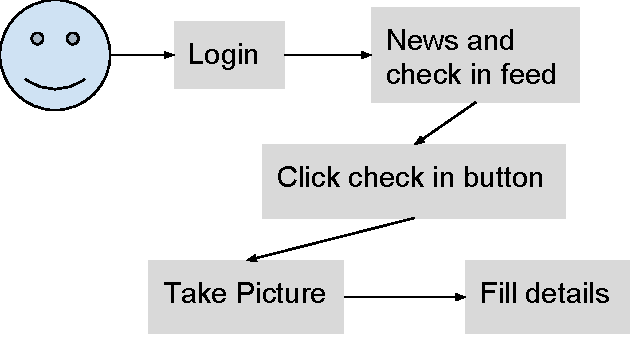
\includegraphics[width=16cm]{pictures/usecasecheckin}

\section{Introduction}


In this assignment we will take a look at the application Untappd. Untappd is an
application designed to accompany drinking, it lets the users check in beer and
rate the beer with a grade of 1 - 5 stars where 5 stars is the best, as well as
keeping tabs and statistics about what you drink and what different types of
beers you have checked in. It also allows companies to see statistics about
their beers. Who drinks it, where is it bought and how much their different
beers are being sold.

\subsection{Goals}

The goals of the assignment is to see how well Untappd performs when used by
users. Among other things, what we intend to find out about the application is
how well it responds to users under the influence of alcohol, which would be
natural for such an application. Is the graphical user interface easy to learn
and able to use efficiently for most people? Even for tipsy people? Is the way
Untappd responds to miss clicks good enough, or is there anything else that
prevents drunk users from using this application. These are some of the major
questions we are going to answer throughout this assignment.

\textbf{List of goals}
\begin{enumerate}
  \item Test and analyze the usability of the application by doing user testing of the application and the functions it contains.
  \item Analyze the application thoroughly by going through the application step-by-step and following Nielsen’s Heuristics.
  \item Create specific use cases and come to conclusion about a possible solution for them.
  Write a conclusion containing a summary of this assessment and possible improvements for Untappd in the feature.
\end{enumerate}

We are going through the goals listed above during this assessment and will try
to explain these as good as possible and also try to go as much into detail
where it may possibly be needed. First of all we are going to explain the
approach we will be taking while evaluating this specific application, Untappd.


\section{Evaluation approach and methods}

The evaluation approach for this assessment will be a bit untraditional. We will
attempt having a user testing while drinking. The reason why we are doing that
is to create the most likely use case for this application, which will therefore
involve drinking beer. This way we will hopefully be able to get some more
realistic results compared to just doing regular testing. This application is
not a necessary piece of technology that society needs, but seems to be a rather
fun or maybe one could say social application that depends solely on the
entertainment and competition it brings to the users. We are intending to see
how this application can affect the already working practices that exist. What
sort of new features does it bring to the users? Is it useful? Will it make an
improvement to the users or the other way around? This and more is something we
will find out by doing the usability tests as mentioned above.


As the user testing will primarily be done by checking in beer, we will also be
evaluating the application after the drunk user testing, in order to achieve
more accurate results. This will include using the heuristics as mentioned
earlier and compare the usability result we got from the “drunk” user testing
with the sober testing in order to be certain that the results are not too much
apart from each other. We will go through all the Nielsen’s heuristics in order
to be able to see how well the application functions all together, and then
summarise the result in the end. This will be done separately from the usability
testing. 

We will also go through a use case with a persona and see the steps needed to do
simple tasks with the app. This way we can illustrate in steps how users
interact with the application
for the tasks.


\section{Practical issues}
 
There are a couple of practical issues that occurred while testing the mobile
application Untappd. This is not something that we didn’t know beforehand, and
is why we still intended to test the application. As Untapped is an application
for checking in different beers, which contains alcohol, the effect of alcohol
might affect the user’s capability of properly using the application the way it
was intended to. However, as the purpose of this assignment was to test and
evaluate the applications usability and performance, it turned out to be a good
way of testing how usable the application turned out to be. If a drunk person is
still able to use an application, then it is more likely to be an easily usable
application.
 
As a user of this application checks in multiple beers, the application might
become somewhat harder to use due to the user’s current state. By that we mean
that the users might not always be as dependable as any other sober person and
the general experience of the application could be different. Therefore, we have
been testing the application both under the influence of alcohol and in a sober
state to make sure that the results seem to somewhat add up.
 
Other than the issue of alcohol affecting how the testing of this application
will be going there are no direct practical issues that we could think of
beforehand other than being able to test the application with a high enough
number of people. We are planning on being the so called “expert users”
according to Nielsen’s Heuristics, but we might also take in consideration other
user tests if they turn out to have some kind of expertise on the subject of
application testing or the content of the application itself.

Taking in consideration that the Untappd application is both an application for
checking in beers and a social platform for people all across the world there
might be difficulties including all of the components needed in order to create
a viable user interface. Speaking from experience, having a high amount of
components in a user interface where space is limited, often tends to create a
kind of messy experience for new users. However, once a user has spent some time
using the application these barriers are often no longer a problem. 




\section{Ethical issues}
The main ethical issues regarding untappd is the encourage consumption of
alcohol. Using and gathering data from this application can pose an undesired disclosure
of information regarding alcohol consumption. We did consider doing a
questionnaire and attempt to get people to submit answers, but since this is
about personal habits, we deemed this hard. Having people to both explain their
drinking habits and if they have used a rather uncommon application such as Untappd
would only provide spare data.


We also chose to do the user testing ourself since we thought it would be hard
find people that would allow us to watch them drink and evaluate an application as this
could we figured it would be uncomfortable for most people.


\section{Evaluation}
As an approach to test the application, we had to take in consideration all the
use cases for the application in order to create an evaluation which was as a
accurate as possible. Therefore, whenever we had a beer we tried to remember to
check in the beers using the application.


Since the application encourages the user to drink beer and cider, which in most
cases contains alcohol, we came to a conclusion that the application would be
used a lot by users heavily under the influence of alcohol, thus we decided that
we had to be that user as well. 


In the end we chose three approaches to analyse and test the application. One,
test the application and check in beers whenever you decide to take a beer. Two,
dedicate a friday night to test the application as much as possible on different
levels of intoxication. And lastly, three, to analyse and test every single
visible component of the application and get user input from people who are not
registered users and have no experience with it whatsoever to see how they
respond to the technology on their first experience with it.




\subsection{Testing levels of intoxication}
Since the app’s consumer market mainly consists of people who drink alcohol, and
is mainly used while consuming alcohol, we decided to test the application
whilst consuming alcohol in order to create a realistic use case. The
application has to be easy to use for people under the influence of alcohol, so
what better way than consuming alcohol ourselves and testing its full potential. 


We all have used the application before, but not a lot, so we already had users in the
application and didn’t to have register. We started simply by heading to “Det
Akademiske Kvarter”, which is a student driven pub and social club in Bergen, we
ordered a Lager pint each and sat down. Even though we had all tasted the
classic Hansa Lager before, we felt we had to include it. After taking a sip of
the cold pint, we unlocked our phones and simply tapped Untapped. When the app
opened it was a pretty straight forward with the same instructions as mentioned
earlier.

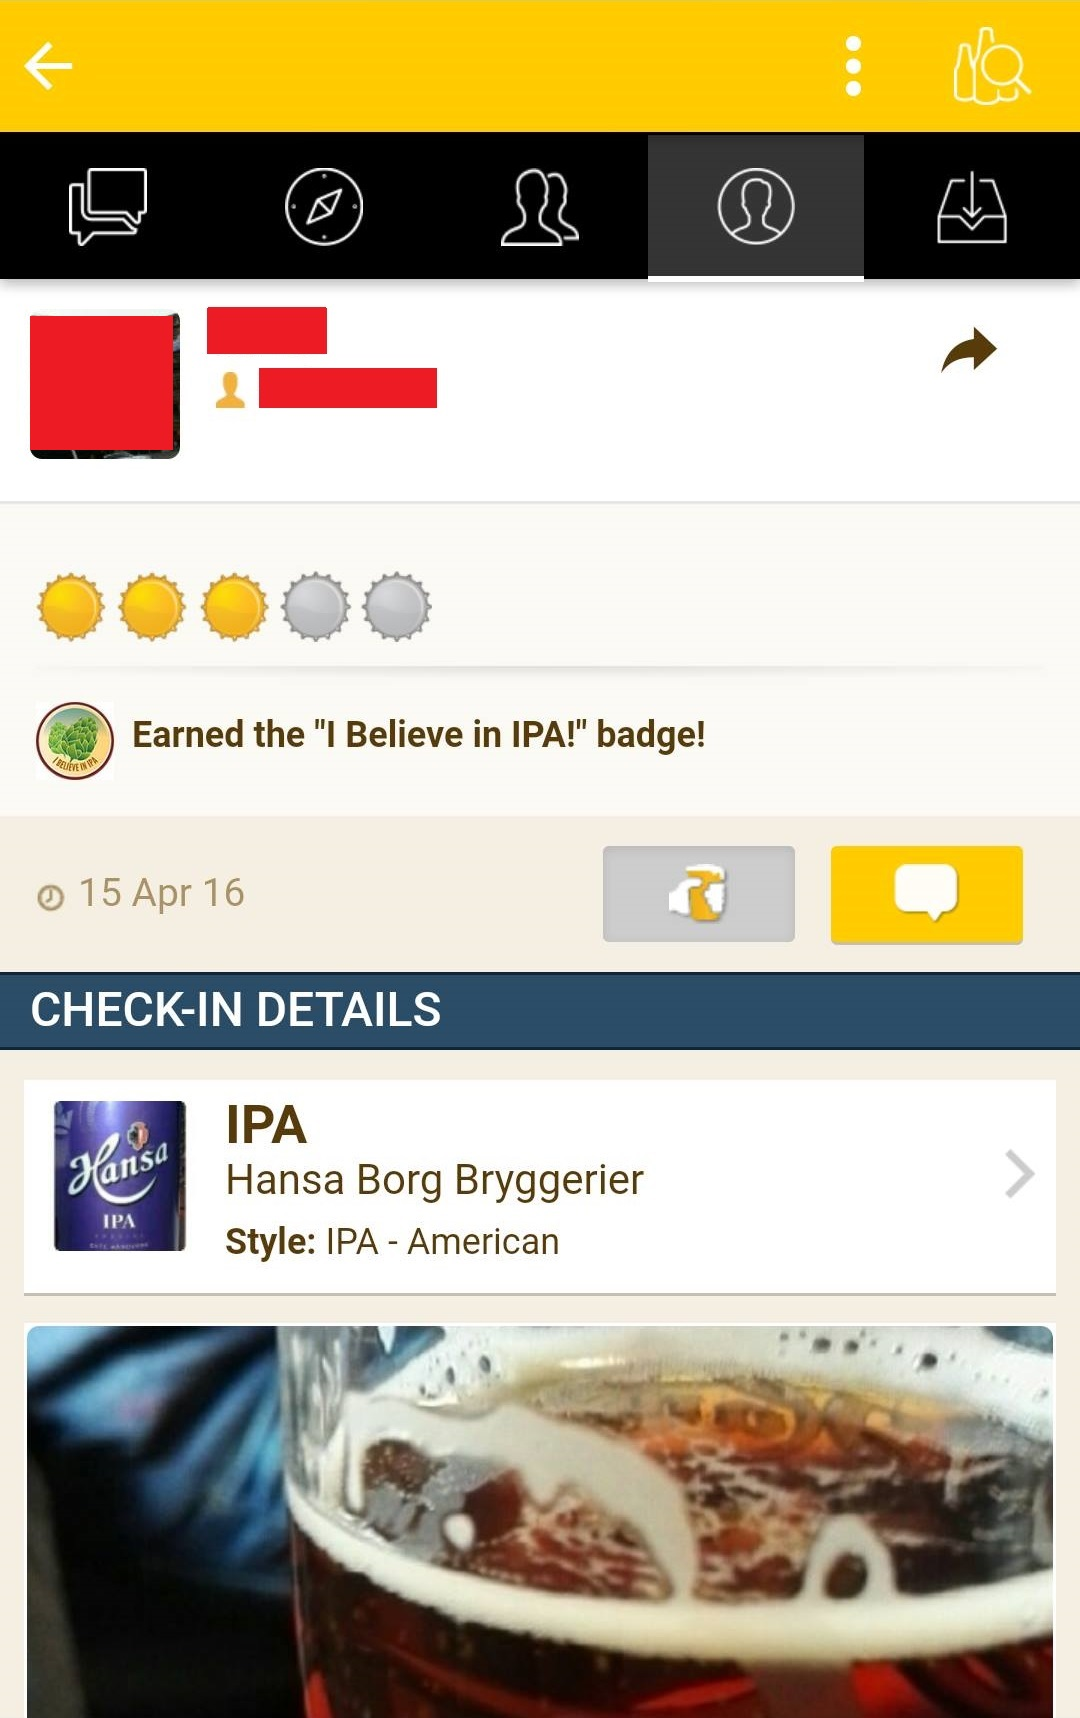
\includegraphics[width=6cm]{pictures/app/sensur1}
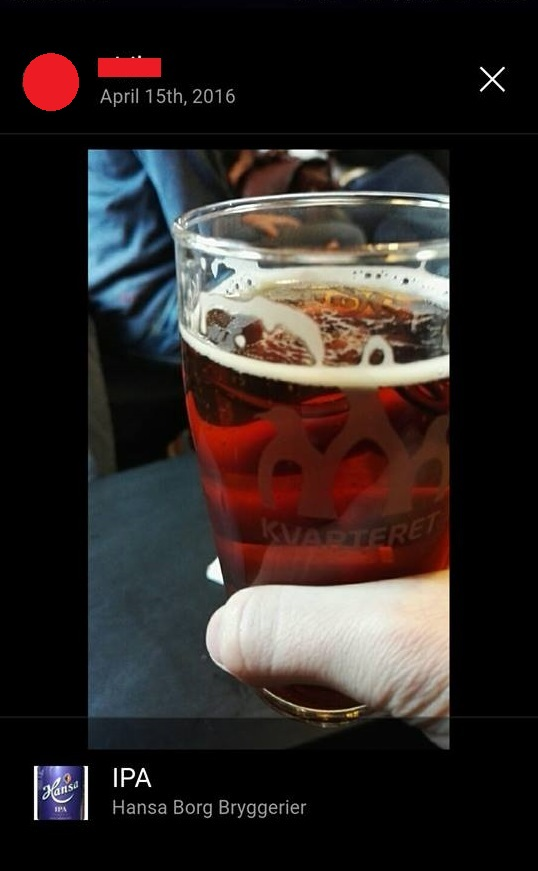
\includegraphics[width=6cm]{pictures/app/sensur2}


We decided to meet some friends for a “vorspiel” and we wanted to continue
testing the app, so we headed to the nearest grocery store and bought
approximately 12 different sorts of beer. We tried to be aware of feeling
affected while testing, but as the night progressed we didn’t really have any
problems using the app, or no problems we could remember at least. When the
night was nearing an end, the application even warned us by giving us a badge,
which is an achievement in the app, that was called “take it easy” and could be
achieved through checking in 12 indistinct beers during one day.


In the end we did not encounter any problems with the application, under the
influence of alcohol. The applications creators most likely designed it to be
used while intoxicated since it kind of encourages the user to drink. However,
even though we managed to use the application while under the influence of
alcohol, doesn't mean it was near perfect. There were several difficulties that
could most likely become problems for a new users of the application. These
issues are both mentioned and discussed below while analyzed using Nielsen’s
heuristics.


\subsection{Nielsen’s heuristics}

In this section we will go through Untappd by using the heuristics created by
Jakob Nielsen.~\cite{usability} to see how well untappd fares with these
requirements.

\subsubsection{Visibility of system status}
When it comes to visibility, the application has a few minor problems. When the user
opens the application, he or she is sent to the main page, on the main page
there are two menus. One of the menus does not say anything, it has simplistic
pictures to visualize what they are but might not be easy to understand. The
second menu is smaller, consisting of only three buttons and does  contain text
but is not necessarily easy to understand. The menu items says “friends, nearby,
groups” but it does not say what it is for. When you select some of the options,
it simply switches the main page feed to the related button, nearby feeds and
friends feeds etc. 

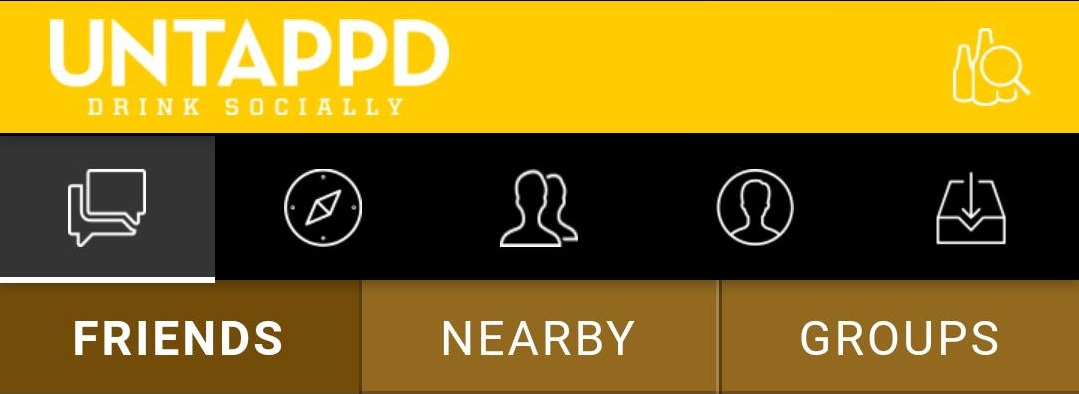
\includegraphics[width=6cm]{pictures/app/manus}
\break
\break
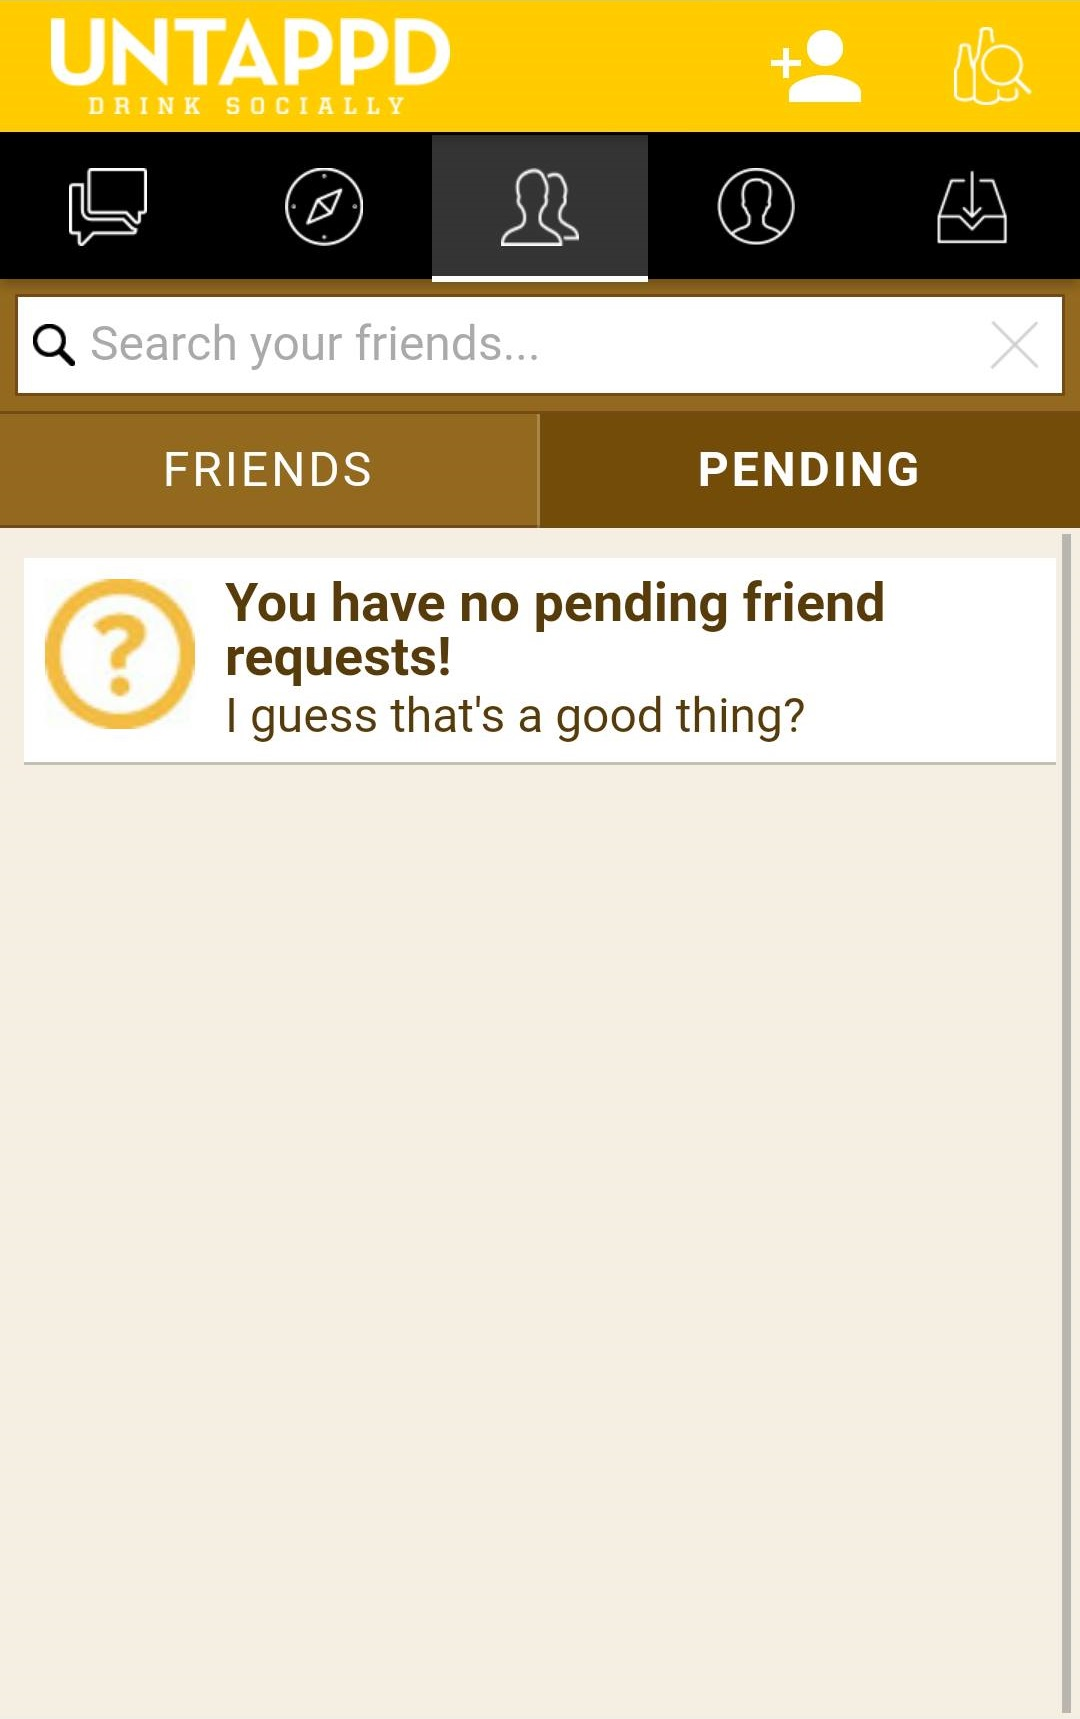
\includegraphics[width=6cm]{pictures/app/pendingfriends}


The first menu, which only contains images, is harder to understand. Some of the
images may be obvious for some users such as the image with two heads, which is
the “Friends” page, and the one with one head being the “Profile” page. However,
for it to be obvious, the user need to have some sort experience from other
applications or programs that have used the same or similar looking pictures or
icons for their menu items. This is not necessarily the case for most new users
and is something that possibly could have been improved. The reason why they are
doing it this way is most likely to avoid using more space than needed as a
mobile screen in most cases can be quite small compared to a computer screen and
they are probably therefore aiming for a better user experience in the long run
instead of an easy start.


The compass icon does not have any real relevance to what it leads to. It leads
to a menu that lets the user select a small number of different categories. Not
beer categories but more like searching and looking for new beer categories. 


Each page of the application has the same layout except for the feed items. On some of
the pages, the menu items were changed. If you look at the screenshot of the app
above, you can see a small illustration in the top right corner, this is a
button for searching for a beer, which is used as the main function for checking
in beers.  When you navigate to different pages, that button is sometimes
removed and replaced with search fields on the page instead and sometimes other
buttons are added to the side of that button. This is something that could be
quite confusing for an intoxicated user. 




\subsubsection{Match between system and the real world}
The application does not contain any language that might not be understood by
the user, taking in precondition that the user does infact speak english. The
closest the application will come to be hard to understand language, is that
each beer has a name and a type, which every user might not understand. But
seeing as the application is focused towards beer enthusiasts, the language is
most likely understandable by the standard user.


Everything is displayed in an orderly fashion, but the beer lists are not sorted
by any clear logic. If the user searches for a beer, it will simply return all
relevant beers with that name somewhere in the description and the user has to
scroll through the lists and keep an eye open. 


\subsubsection{User control and freedom}
As for undo and redo, it does not have any indistinct “Back” or “Home” buttons.
Most of the items used for navigation is in the menu and can be accessed on
every page. If the user happens to press “Back” on a OS native button on the
phone, he or she can simply tap the menu item that they were using and be sent
back to where they were and it does not remove whatever they were doing on that
page. 


Even though the application does not have a “redo” button, it is very easy to redo
actions when misclicking something. If the user has, for instance, been to the
“Friends” panel and tapped “Pending” and then returned home, he or she can
simply tap the “Friends” panel and automatically be returned to the “pending”
panel on tap.  


\subsubsection{Consistency and standards}
There should be no trouble navigating for the user when looking at buttons and
reading words. The are no buttons that has the same name or same illustration,
so it should not be any problem understanding what is going on. 


There is one small problem though. If the user is on the main page, and has
selected “Nearby” to look what nearby people have checked in and then started
navigating other places in the app, the main page would still be on the “Nearby”
section which might cause confusion when returning to the main page since the
only way of truly knowing the difference between the pages is by looking at the
color of the menu. This might cause some confusion but is not a hard fix, by the
simple tap of a button the user can return the menu to however he or she
prefers. 


In addition to this, there is a button right next to the search button up in the
top right corner which only appears only if certain other tabs are selected.
While checking out your profile this icon will appear as something that might
look like a settings icon and if you are currently viewing friends this icon
becomes an icon of a person and a + sign which might indicate an add friend
button. This is a good way of saving space, but could be confusing to begin
with. One of the main functions however, the search button for finding beers is
constantly placed in the top right corner and does not depend on anything else
being selected to use it which is good. 


\subsubsection{Error prevention}
The only error we have encountered with the app, is the loss of connection which
simply states “Error You don’t appear to have network connection. Please check
your connection and try again.” with an OK button at the end. This is not a
problem with the app, it simply reminds the user that the wifi on the phone is
either turned off or there is some sort of problem outside the app. 


Neither friends or family, or friends of friends has ever had any complaints
about errors through the app. The application has a good design that prevents errors
from occurring  as there does not seem to be too many actions that could end up
in an error being thrown. 


\subsubsection{Recognition rather than recall}
The application has had its moments when it comes to performance. The search functions
and load functions of the application are all as fast as lightning. The user does not
have to wait or do other things while waiting for actions to happen on the app. 


Even though the application is fast and does not take too much of the user's time, it
has crashed a couple of times for different users. This is most likely because
of the difference in phones and specs between each user. Some users has had
minor crashing problems, but has blamed the phone not the application itself.
According to users who has seen the application crash on their phone it is because “The
phone often quits apps and performs poorly”, thus nobody has blamed the
application for crashing. 


\subsubsection{Flexibility and efficiency of use}
Untappd has a pretty straightforward menu system. One bar for the main features
of the app, and the top row for a back button, more options and a check in
button. This makes it very efficient for the user to walk through all the main
components of the app. The one complaint could be the placement of the check in
button. The button is placed in the upper right corner of the screen. This makes
the button hard to reach when holding the phone in the left arm and using the
thumb.


One solution to this problem could be to place it in a lower corner where it
does not obstruct the layout. The current placement could be intentional to
prevent users from entering the check in screen by accident. There are also
applications allowing you to scan barcodes or the etiquette of the product. A
solution along the lines of this could help Untappd to be easier to use for
people searching the beer, and they could always default back to the search bar
if nothing is found.


Apart from that, the interface is easy enough that adding new features could be
done easily with the current layout. There is not much bloat in the interface
and its sleek and polished.




\subsubsection{Aesthetic and minimalist design}
The application does not contain or display much unnecessary information. Instead of
texted menus, the application uses relevant illustrations for the different pages, even
though not all menu illustrations are very relevant. The application keeps a simple
style and does not crop too much information on the screen. It keeps a clean
look while providing all the information the user needs. The only instance where
the users does not receive all the information he or she needs is in the one
menu item that resembles a compass but provides categories.  The application has
a good and minimalistic design all in all as they have used the space they have
to deal with good and provide the needed information for each specific
situation. An example for this is the menu items which all has their own
submenus containing more options or information about the specific item.


\subsubsection{Help and documentation}
The application also provides relevant and helpful guides for different actions. The
main function of the app, checking in beer, has a list of useful guides for the
user to better learn and understand the process of what he or she wants to do.
When navigating to checking in a beer, The application displays a little box the first
time the user enters the page, saying “More information above” and pointing to
the three dots on the top of the menu. When tapping the menu, different guides
will pop up and the user can choose the one most relevant to his or her need. 
  
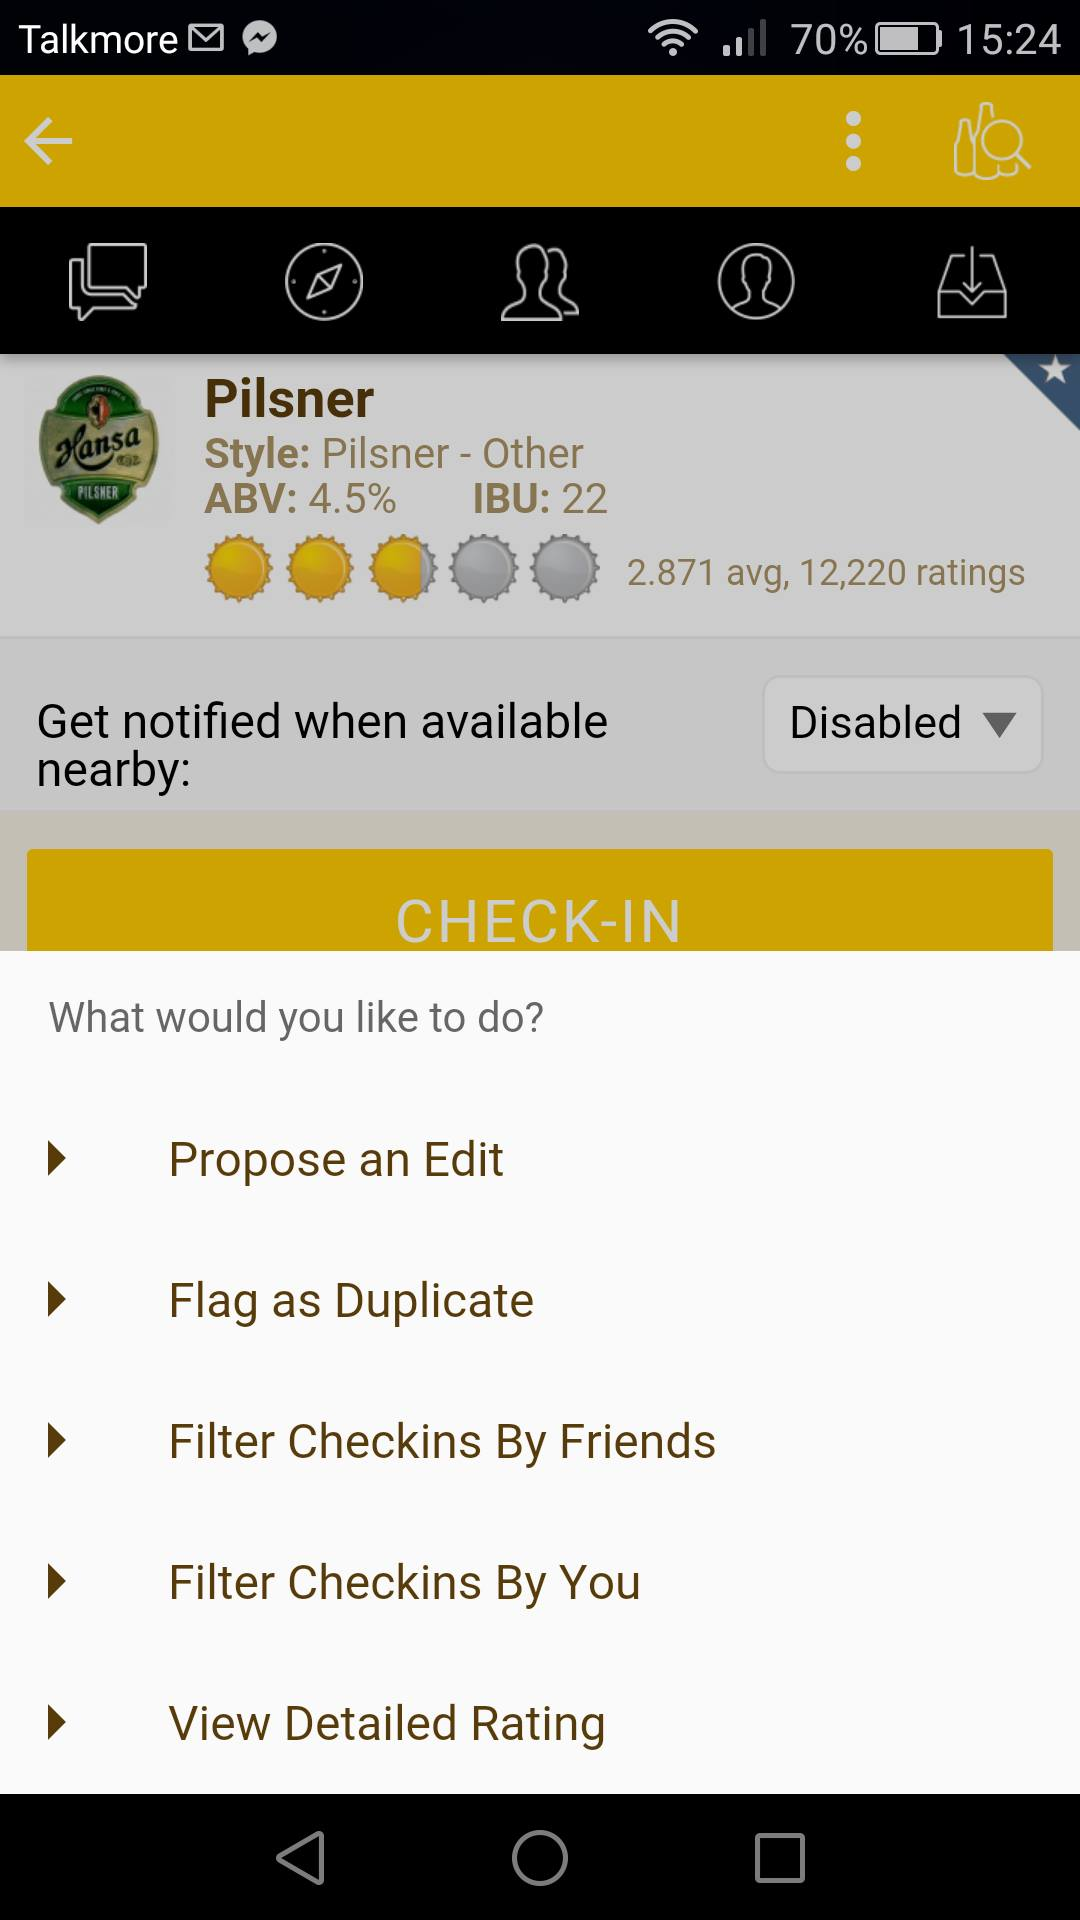
\includegraphics[width=6cm]{pictures/app/help}

\subsection{Use case and requirements}
The app’s goal is to make the user share their ideas of good beer with other
users. Since it forces the user to create a user before using the app, it is
likely that the creators of the application wants to create a personal community amongst
the beer enthusiasts. 


Use cases attempts to highlight the steps needed to complete a given task in a
system, in this case, an mobile application.\cite{usecase} Doing this we can test and highlight
possible flaws in the UI. In this use case we will go through each step of how
the user can view other user's beer recommendations.

\textbf{Use Case:} View other users and their recommendations. 

\textbf{Actor:} Registered User

\textbf{Overview:} The user opens the application and finds a song to play. The user
taps a song under ‘recent songs’ and is navigated to an info page about the
song. The user deselects ‘competitive’ mode and hits play. The song starts
playing and the chords drop down. When the song is over, the user is navigated
to a page where he/she can rate, comment and favorite the song. The user can
then either play the song again or return home to find a new song to play.

\begin{enumerate}[leftmargin=-0in]
  \item[] \textbf{Preconditions:} 
    \begin{itemize}
      \item The user has already registered and logged in.
    \end{itemize}
\end{enumerate}
\begin{itemize}[leftmargin=-0in]
  \item[] \textbf{Basic flow:} Find another users beer recommendations.
  \item[] \textbf{Description:} The user wants to find new beer to taste, and is
    going to check out other users recommendations.
    \begin{enumerate}
      \item Open the app.
      \item Tap the middle icon on the menu, which is the friends icon.
      \item Tap one of the friends on the list.
      \item Scroll down on the selected friends wall.
      \item Tap one of the beers and read up on it.
      \item Done. 
    \end{enumerate}
\end{itemize}
\textbf{Termination Outcome:} The user has now found a new beer to taste through
another users recommendations.


\begin{itemize}[leftmargin=-0in]
  \item[] \textbf{Alternative Flow 3A:} The user has no friends.
  \item[] \textbf{Description:} If the user navigates to the friends panel and
    has no friends, he will get no users to browse.
    \begin{enumerate}
      \item Tap the compass icon, second to the left on the menu.
      \item Tap either “Trending Beers”, “Top rated Beers”, “Nearby Beers” or “Global Feed” 
      \item Scroll down the wall of either of the selected categories.
      \item Tap one of the beers and read up on it.
      \item Done.
    \end{enumerate}
\end{itemize}
\textbf{Termination Outcome:} The user has found new beers to taste even though he or she has no friends to get recommendations from.


\section{Conclusion}
The application could be more descriptive on some fronts. Menus and buttons
could make more sense so that the user won’t have to tap a button to test what
happens and then tap return. The etiquette checker could also be a nice addition
on the application itself. But overall the application was easy to use and
surprisingly easy to use for a user under the influence, which it should be.
Untappd scores with its rather good interface and easy to access social media
features. A few things could maybe be placed different, like the check in
button. But this is overall minor issues with the application.

Despite its ethical dilemmas, Untapped is a great tool for both beer lovers and
beer breweries. The users can share their opinions and get recommendations while
the breweries can take in consideration the opinions and ratings from the users
in making better beer.


\clearpage
\bibliography{oppgave}
\bibliographystyle{plain}

\end{document}
